% Created 2022-07-03 Sun 15:51
% Intended LaTeX compiler: pdflatex
\documentclass[smaller]{beamer}
\usepackage[utf8]{inputenc}
\usepackage[T1]{fontenc}
\usepackage{graphicx}
\usepackage{longtable}
\usepackage{wrapfig}
\usepackage{rotating}
\usepackage[normalem]{ulem}
\usepackage{amsmath}
\usepackage{amssymb}
\usepackage{capt-of}
\usepackage{hyperref}
\usepackage{verbatim, multicol, tabularx}
\usepackage{sourcecodepro}
\usepackage[T1]{fontenc}
\usepackage{amsmath,amsthm, amssymb, latexsym, listings, qtree, tikz}
\lstset{extendedchars=\true, inputencoding=utf8, frame=tb, aboveskip=1mm, belowskip=0mm, showstringspaces=false, columns=flexible, basicstyle={\footnotesize\ttfamily}, numbers=left, frame=single, breaklines=true, breakatwhitespace=true, tabsize=4,  keywordstyle=\color{blue}, identifierstyle=\color{violet}, stringstyle=\color{teal}, commentstyle=\color{darkgray}}
\setbeamertemplate{footline}[frame number]
\hypersetup{colorlinks=true,urlcolor=blue}
\usetheme{default}
\date{}
\title{Sets}
\hypersetup{
 pdfauthor={},
 pdftitle={Sets},
 pdfkeywords={},
 pdfsubject={},
 pdfcreator={Emacs 28.1 (Org mode 9.5.2)},
 pdflang={English}}
\begin{document}

\maketitle

\section{Sets}
\label{sec:org2a5e530}

\begin{frame}[label={sec:org5da47d1}]{Sets}
Collection of elements.

\begin{itemize}
\item Empty set: \(\varnothing\)
\item Integers: \(\mathbb{Z}\)
\item Natural numbers: \(\mathbb{N}\)
\item Real numbers: \(\mathbb{R}\)
\item Rational numbers: \(\mathbb{Q}\)
\end{itemize}
\end{frame}

\begin{frame}[label={sec:org1e6eb2d}]{Cartesian Product}
ordered paris of elements from multiple sets
\end{frame}

\begin{frame}[label={sec:orgc263bde}]{Subsets}
If \(A \subseteq B\), then no element of \(A\) is not in \(B\).
\end{frame}

\begin{frame}[label={sec:orgc1147e8}]{Power Sets}
Powerset of \(A\), \(\mathcal{P}(A)\) is the set of all subsets of \(A\).  There are \(2^{|A|}\) subsets of \(A\).
\end{frame}

\begin{frame}[label={sec:org586b165}]{Set Union}
Like OR.  \(A \cup B\) is a set of all elements of either \(A\) or \(B\).
\end{frame}

\begin{frame}[label={sec:orgf75a389}]{Set Intersection}
Like AND.  \(A \cap B\) is the set of all elements that are in in both \(A\) and \(B\).
\end{frame}

\begin{frame}[label={sec:org84bacbe}]{Set Difference}
\(A - B\) is the set of all things in \(A\) that are not in \(B\).
\end{frame}

\begin{frame}[label={sec:org5de9439}]{Complement}
Universal set, aka, universe of discourse, \(U\).

Complement of \(A\), \(\overline{A}\), is the set \(U - A\).
\end{frame}

\begin{frame}[label={sec:orgcd860c6}]{Venn Diagrams}
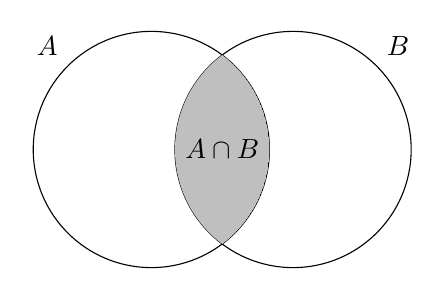
\begin{tikzpicture}

% Set A
\node [draw,
    circle,
    minimum size =3cm,
    label={135:$A$}] (A) at (0,0){};

% Set B
\node [draw,
    circle,
    minimum size =3cm,
    label={45:$B$}] (B) at (1.8,0){};

% Intersection
\begin{scope}
    \clip (0,0) circle(1.5cm);
    \clip (1.8,0) circle(1.5cm);
    \fill[lightgray](0,0) circle(1.5cm);
\end{scope}

% Set intersection label
\node at (0.9,0) {$A\cap B$};

\end{tikzpicture}
\end{frame}


\begin{frame}[label={sec:org7c6d325}]{Proofs}
\begin{itemize}
\item Proofs are chains of statements that lead from axioms to a final statement, called a conclusion, such that if each statement in the proof is true, the conclusion must be true.
\end{itemize}

\begin{alertblock}{Truth}
Mathematical logic does not deal with the meaning of truth.  It only deals with the systematic treatment of true and false statements.  The meaning of truth is a matter for philosophy.
\end{alertblock}
\end{frame}

\begin{frame}[label={sec:org968359c}]{Theorems}
\begin{itemize}
\item Theorems are statements that have been proved.
\begin{itemize}
\item We usually use \emph{theorem} to refer to major results in mathematics.
\end{itemize}
\item Lemmas are theorems that are useful primarily in proving other theorems.
\item Corrollaries are theorems that follow "quickly" (one or two deduction steps) from a theorem.
\end{itemize}
\end{frame}

\begin{frame}[label={sec:org48625da}]{Example: Context-free Grammars}
Consider the following system of axioms:

\begin{itemize}
\item \(S \rightarrow aSb\)
\item \(S \rightarrow \epsilon\), where \(\epsilon\) means empty string
\end{itemize}

The set of axioms above is in instance of a \emph{grammar}.  A grammar is

\begin{itemize}
\item a set of \emph{terminal symbols}, which can be an \emph{alphabet} (a.k.a. \emph{lexicon}) or set of words; here \(\{a, b\}\),
\item a set of \emph{nonterminal symbols} which act as syntactic vairables in the grammar; here \(\{S\}\),
\item a distinguished nonterminal that acts as the start symbol; here \(S\), and
\item a set of axioms of the form \(\alpha \rightarrow \beta\), called \emph{production} or \emph{grammar} rules.
\end{itemize}

A \emph{context-free grammar} contains production rules with only nonterminals on the left.
\end{frame}

\begin{frame}[label={sec:orge9d1c04}]{Example: Language Generation}
A production rule says that the symbol on the left can be replaced by the sequence of symbols on the right.  A sequence of subsititions consitutes a \emph{proof} that the final sequence of symbols, the conclusion, is a sentence in the language specified by the grammar.  For example


\begin{center}
\begin{tabular}{ll}
\(S\) & the start symbol\\
\(aSb\) & by Rule 1, \(S \rightarrow aSb\)\\
\(aaSbb\) & by Rule 1, \(S \rightarrow aSb\)\\
\(aabb\) & by Rule 2, \(S \rightarrow \epsilon\)\\
\end{tabular}
\end{center}

is a proof that the sequence of symbols, or \emph{string}, \(aabb\) is a sentence of the language, generated by successive applications of axioms, or production rules, in the langauge's grammar.

\begin{alertblock}{Parsing}
The opposite problem, determining whether a given string is a valid sentence in a language, can be solved by finding a sequence of production rules that produce the string.  This sequence of production rules can be represented as a tree, called a \emph{parse tree}, and the program that does this is called a \emph{parser}.  A parser is an essential component of language analyzers such as interpreters and compilers.
\end{alertblock}
\end{frame}

\begin{frame}[label={sec:org0eec51d}]{Truth Functionals}
An assignment of true or false to a new proposition is \alert{truth functional} if the assignment is made based on the truth of related propositions, and the validity of the logical connectives linking the component propositions to the new proposition.  In other words, the truth of a proposition is a \emph{function} of the truth values of logically related propositions.
\end{frame}
\end{document}